\section{The Neural code}
\exm Assuming that the neural response and its relation to the stimulus are completely characterized by the probability distribution of spike times as a function of the stimulus. If spike generation can be described as an inhomogeneous Poisson process, this probability distribution can be computed from the time-dependent firing rate r($t$),  using equation 1.37. In this case, r($t$) contains all the information about the stimulus that can be extracted from the spike train, and the neural code could reasonably be called a rate code.
\rem The central issue in neural coding is whether individual action potentials and individual neurons encode independently of each other, or whether correlations between different spikes and different neurons carry significant amounts of information.
\subsection{Independent-Spike,Independent-Neuron,and Correlation Codes}
\rem All information in this section refers to stimulating information.
\defn [\emph{Independent-Spike Code}]A code based solely on the time-dependent firing rate. This refers to the fact that the generation of each spike is independent of all the other spikes in the train.
\defn [\emph{Correlation Codes}]Individual spikes do not encode independently of each other, correlations between spike times may carry additional correlation code information.
\rem It has been found that some information is carried by correlations between two or more spikes, but this information is rarely larger than 10$\%$ of the information carried by spikes considered independently.Information could be carried by more complex relationships between spikes.Independent-spike codes are much simpler to analyze than correlation codes, and most work on neural coding assumes spike independence.
\rul Information is typically encoded by neuronal populations.
\rem We still consider whether individual neurons act independently, or whether correlations between different neurons carry additional information.
\rem The analysis of population coding is easiest if the response of each neuron is considered statistically independent.It means that they can be combined without taking correlations into account.
\defn [\emph{Independent-Neuron Code}]\emph{Independent-neuron code} means the response of each neuron in a neural population is considered statistically independent.
\rem The assumption of independent-neuron coding is a useful simplification that is not in gross contradiction with experimental data, but it is less well established and more likely to be challenged in the future than the independent-spike hypothesis.
\rem To test the validity of independent-neuron, we should know whether correlations between the spiking of different neurons provide additional information about a stimulus that cannot be obtained by considering all of their firing patterns individually.
\prin Synchronous firing of two or more neurons and rhythmic oscillations of population activity are mechanism for conveying information in a population correlation code.
\exm Place-cell coding of spatial location in the rat hippocampus, which at least some additional information appears to be carried by correlations between the firing patterns of neurons in a population. The firing rates of many hippocampal neurons, recorded when a rat is moving around a familiar environment, depend on the location of the animal and are restricted to spatially localized areas called the place fields of the cells. When a rat explores an environment, hippocampal neurons fire collectively in a rhythmic pattern with a frequency in the theta range, 7-12 Hz. The spiking time of an individual place cell relative to the phase of the population theta rhythm gives additional information about the location of the rat not provided by place cells considered individually.
\begin{center}
    \label{fig:1.18}
    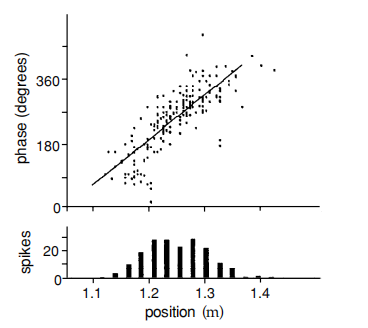
\includegraphics[scale = 0.5]{./png/Figure1-18}\\
\end{center}
Each dot in the upper figure shows the phase of the theta rhythm plotted against the position of the animal at the time when a spike was fired. The linear relation shows that information about position is contained in the relative phase of firing. The lower plot is a conventional place field tuning curve of spike count versus position.

\subsection{Temporal Codes}
\rul Precise spike timing is a significant element in neural encoding. When precise spike timing or high-frequency firing-rate fluctuations are found to carry information, the neural code is often identified as a temporal code.
\rem The temporal structure of a spike train or firing rate evoked by a stimulus is determined both by the dynamics of the stimulus and by the nature of the neural encoding process. Stimuli that change rapidly tend to generate precisely timed spikes and rapidly changing firing rates.
\rem Temporal coding refers to temporal precision in the response that not only arise from the dynamics of the stimulus but also relates to properties of the stimulus.
\rul If the independent-spike hypothesis is valid, the temporal character of the neural code is determined by the behavior of r(\emph{t}).
\defn If r(\emph{t}) varies slowly with time, the code is typically called a \emph{rate code}, and if it varies rapidly, the code is called \emph{temporal code}.
\exm Different firing-rate behaviors for a neuron in area MT of a monkey recorded over multiple trials with three different stimuli(consisting of moving random dots). The activity in the top panel would typically be regarded as reflecting rate coding, and the activity in the bottom panel as reflecting temporal coding.
\begin{center}
    \label{fig:1.19}
    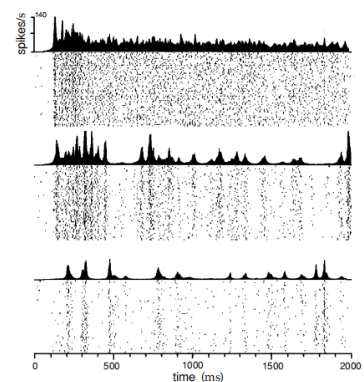
\includegraphics[scale = 0.6]{./png/Figure1-19}\\
\end{center}

\rem It is not obvious what criterion should be used to characterize the changes in r(\emph{t})as slow or rapid. The identification of rate and temporal coding in this way is ambiguous.
\exm Using the spikes to distinguish slow from rapid, so that a temporal code is identified when peaks in the firing rate occur with roughly the same frequency as the spikes themselves. In this case, each peak corresponds to the firing of only one, or at most a few action potentials.
\rem When many neurons are involved, any single neuron may fire only a few spikes before its firing rate changes, but the population may produce a large number of spikes over the same time period. Thus, it is not targeted at populations.
\exm Using the stimulus to establish what makes a temporal code. In this case, a temporal code is defined as one in which information is carried by details of spike timing on a scale shorter than the fastest time characterizing variations of the stimulus. This requires that frequencies higher than those present in the stimulus.
\rul A temporal code has been reported when using spikes to define the nature of the code, and it would be called rate codes if the stimulus
were used instead.


%%% Local Variables:
%%% mode: latex
%%% TeX-master: t
%%% End:





